\section{Results}

\subsection{Robust Predictive Performance Across Hydrological Stations}

Interpretability analysis is most meaningful when the underlying predictions are reasonably accurate. We therefore first verify that STEH achieves reliable predictive performance across hydrological stations\cite{ReviewOfXAI}. Predictive skill is evaluated using the NSE, and we follow the commonly used threshold of NSE $>$ 0.5 to indicate satisfactory performance\cite{Nse}.

\begin{figure}[ht]
    \centering
    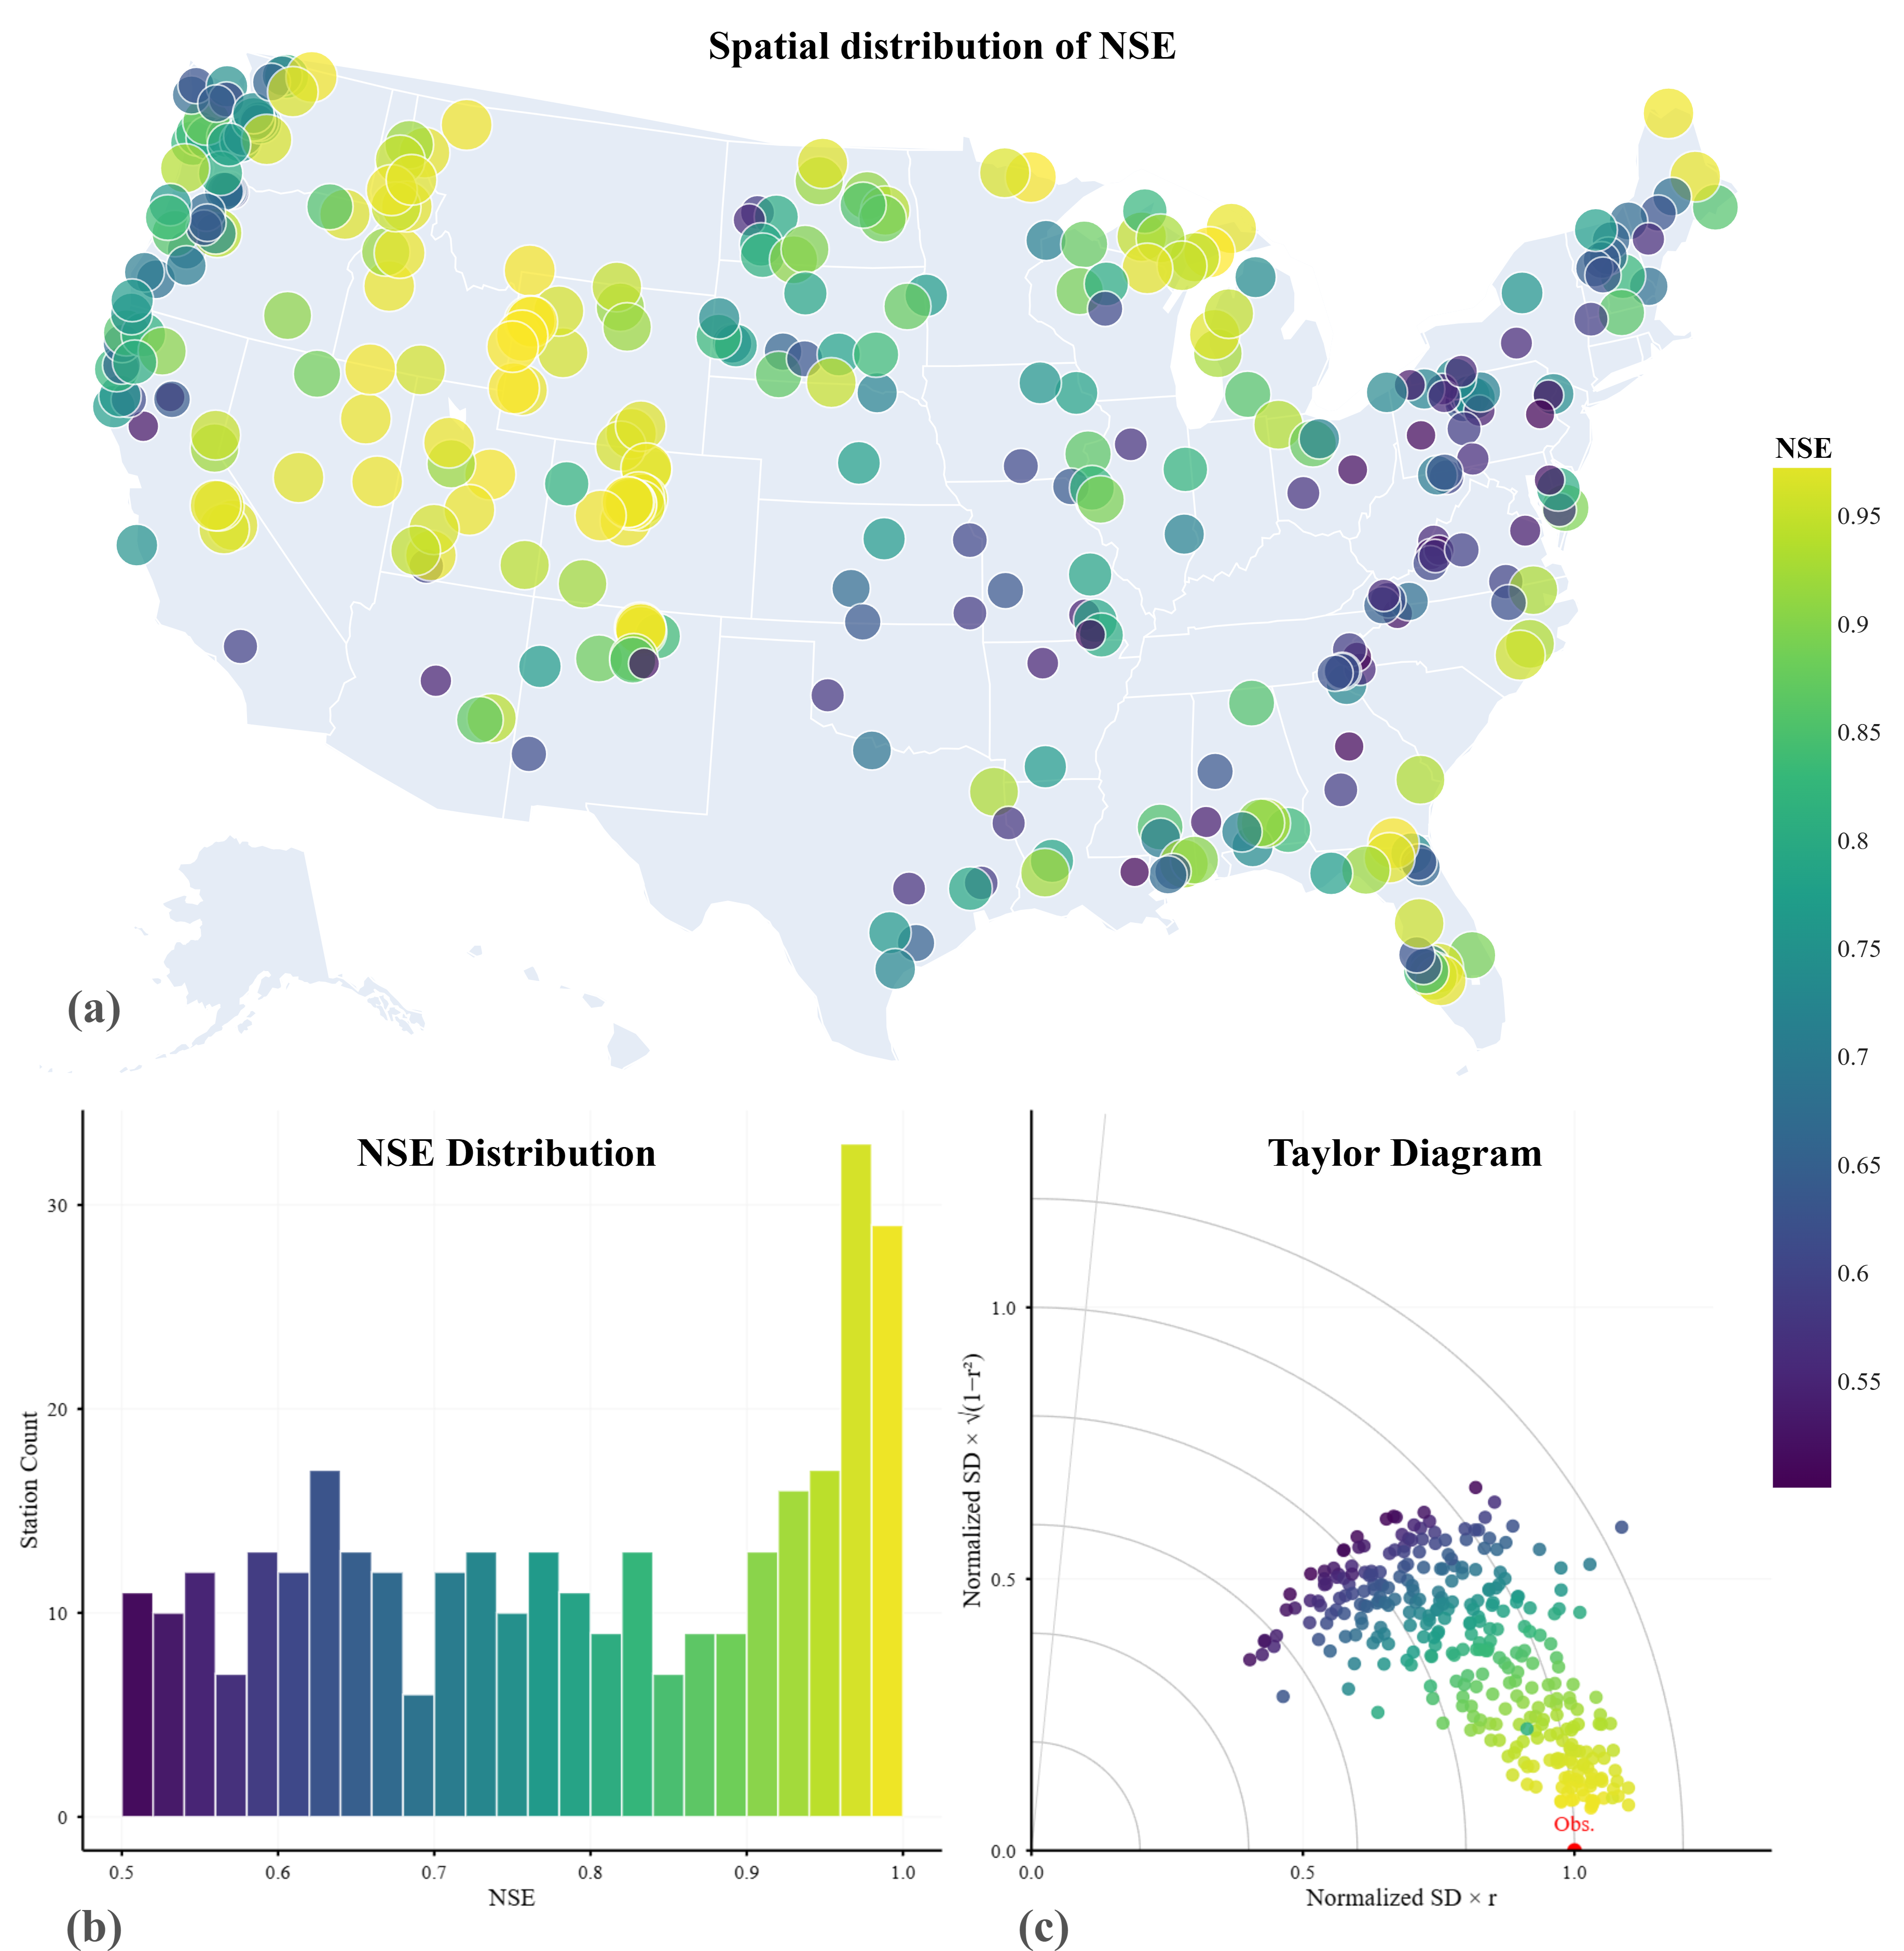
\includegraphics[width=\textwidth]{../Figures/Fig3 Model Prediction.png}
    \caption{\textbf{Model performance across 521 streamflow gauging stations.} (a) Spatial distribution of NSE, with warmer colors indicating higher predictive skill. (b) Distribution of NSE values across all stations, showing that the majority achieve satisfactory performance (NSE $>$ 0.5). (c) Taylor diagram summarizing model performance in terms of correlation, normalized standard deviation, and centered root-mean-square error relative to observations. Overall, the results indicate that the model provides robust predictions for a large proportion of stations, while performance varies across regions, reflecting differences in hydrological conditions.}
    \label{nseDistribution}
\end{figure}


As shown in Fig.~\ref{nseDistribution}, STEH achieves satisfactory skill for a large proportion of stations, even though it is designed to prioritize interpretability rather than purely optimizing predictive accuracy. Specifically, 327 out of 521 stations (approximately 62.8\%) achieve NSE values greater than 0.5\cite{WRR_RMSE}.

These results indicate that the model captures key hydrological dynamics in many basins\cite{WRR_NSE}, providing a practical foundation\cite{ReviewOfXAI} for the subsequent interpretability analyses. The insights reported below are therefore grounded in meaningful predictive behavior rather than artifacts of uniformly poor performance\cite{hess-camels}. We next investigate the learned circuit structures and pathways.

\FloatBarrier

\subsection{Interpretable Circuit Structures Across Hydrological Stations}
Given the large number of stations (521), it is impractical to visualize the learned circuits for all stations individually. Therefore, a representative sampling strategy is adopted to systematically examine circuit structures under different predictive conditions.

Specifically, stations are categorized into three performance groups\cite{Nse} based on the NSE. One representative station is selected from each category, as summarized in Table~\ref{tab:nse_categories}.

\begin{table}[htbp]
    \centering
    \caption{Representative stations across NSE performance categories}
    \label{tab:nse_categories}
    \begin{tabular*}{\textwidth}{@{\extracolsep{\fill}}lccc}
        \toprule
        Performance Category & NSE Range & Station ID & NSE \\
        \midrule
        Very Good     & NSE $>$ 0.75              & 09066300 & 0.9905 \\
        Good          & 0.65 $<$ NSE $\leq$ 0.75 & 01439500 & 0.7366 \\
        Satisfactory  & 0.50 $<$ NSE $\leq$ 0.65 & 03504000 & 0.6217 \\
        \bottomrule
    \end{tabular*}
\end{table}

We first consider a representative inland station with very good performance (Station ID: 09066300, \textit{Middle Creek near Minturn, CO.}, 39.65°N, 106.38°W, NSE = 0.9905) to illustrate the extracted core circuit (Fig.~\ref{fig:inland_circuit}). The station is located in a high-altitude inland basin in Colorado, USA (approximately 3251 m), where hydrological processes are strongly influenced by temperature-driven dynamics and catchment routing\cite{Biemans2019}.

The circuit structure (Fig.~\ref{fig:inland_circuit}a) shows that the model retains a clear and stable information flow pathway after strong sparsification. Among the inputs, streamflow (Q) and maximum temperature (Tmax) dominate, with substantially stronger connections than DayL. Beyond variable importance, this structure suggests a process-level pattern in which antecedent catchment state (with Q acting as a storage proxy) and temperature jointly regulate runoff release. The recovered pathway is consistent with plausible high-altitude controls such as snowmelt timing and evapotranspiration sensitivity\cite{openai_weight_sparse_transformers}. Within the hidden layers, information propagates through a small number of key nodes and converges to the output, forming a compact, low-redundancy computational pathway.

Training dynamics (Fig.~\ref{fig:inland_circuit}a, lower right) provide complementary evidence: as the number of retained nodes (K) increases, NSE rapidly improves to near 1 and stabilizes when K remains relatively small (K < 100), while MSE decreases sharply and stays low. Notably, performance comparable to the full model is achieved with only a small subset of nodes. This indicates that the extracted sparse circuit preserves essential predictive capability, supporting its functional fidelity\cite{NIPS2015_three_step_pruning}. More broadly, the sparsity-inducing training appears to retain critical computational units while removing redundant structure\cite{wang2022interpretabilitywildcircuitindirect}.

Furthermore, the interaction analysis (Fig.~\ref{fig:inland_circuit}b) reveals strong dependencies among input variables. In particular, Tmax exhibits the strongest interaction with Q, followed by the interaction between Q and DayL, while DayL shows relatively weak interactions overall. This supports a process-level interpretation: thermal forcing does not act independently, but modulates discharge response through antecedent-state conditioning, consistent with energy-state coupling in mountain basins\cite{WRR_shap}.

Finally, the contribution analysis (Fig.~\ref{fig:inland_circuit}c) shows a clear imbalance among input variables. Streamflow (Q) contributes the most, followed by Tmax, while DayL has the smallest contribution. Combined with the circuit and interaction evidence, this indicates that the dominant hydrological pattern at this site is a state-dependent runoff pathway with secondary temperature regulation, rather than a uniformly distributed multi-driver response.

Overall, for this very good inland station, the extracted core circuit is highly sparse while maintaining strong predictive capability\cite{7552539}. More importantly, STEH recovers a coherent hydrological mode in which antecedent state and thermal forcing jointly govern streamflow response, suggesting that the learned sparse circuit reflects hydrologically meaningful structure rather than only statistical attribution.

\begin{figure}[ht]
    \centering
    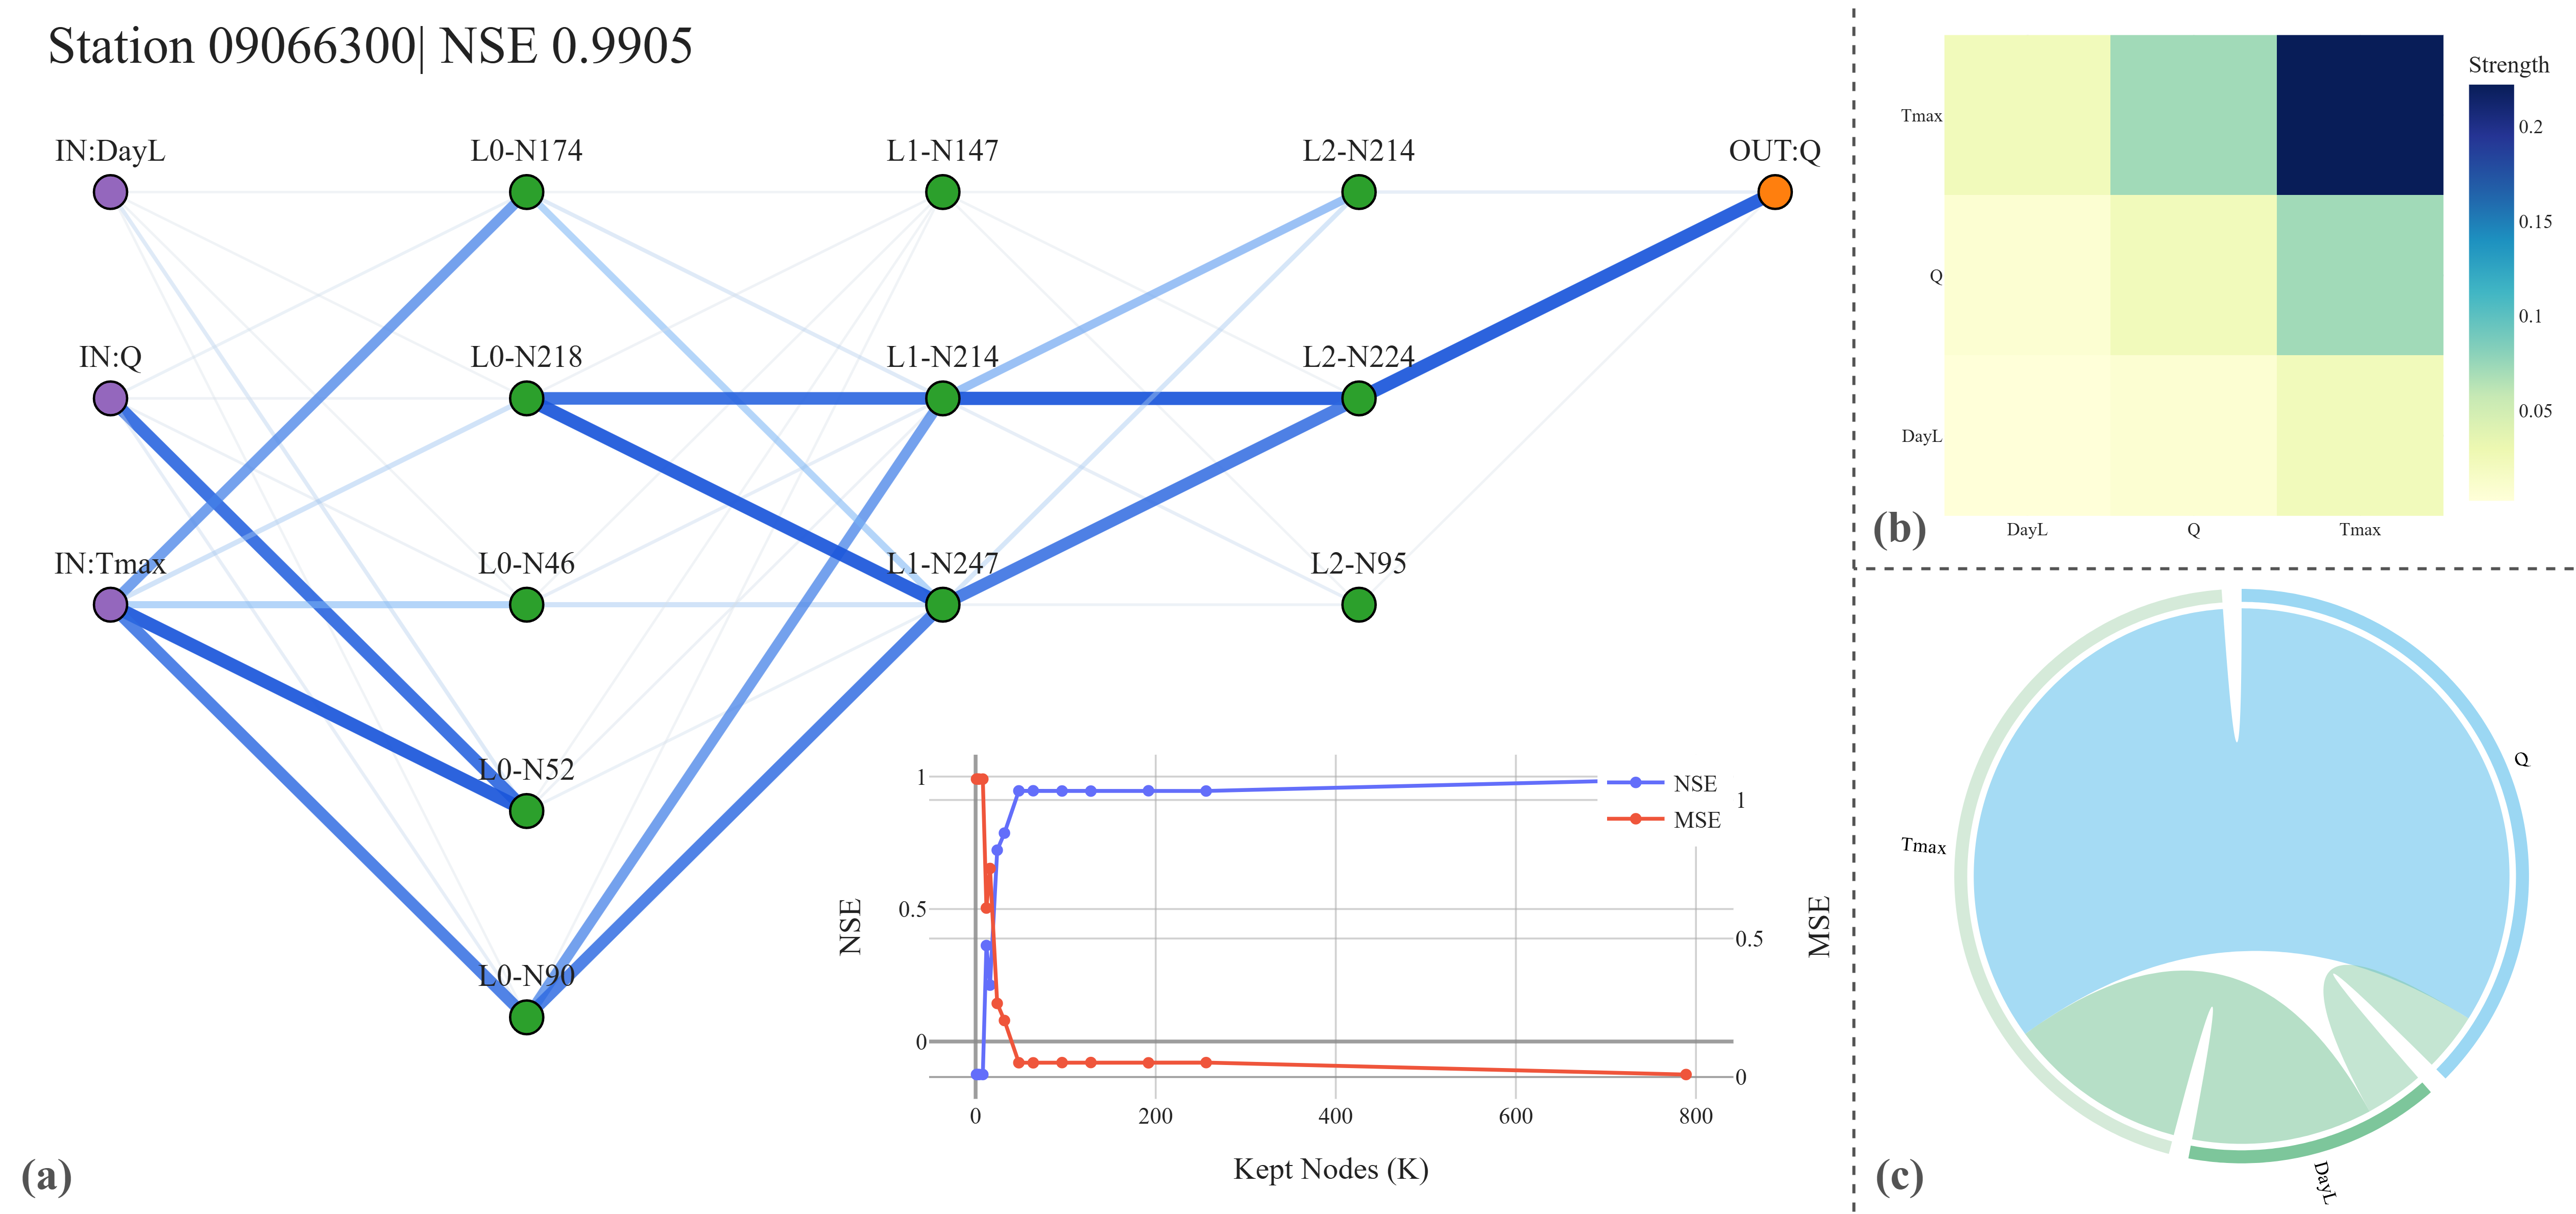
\includegraphics[width=\linewidth]{../Figures/Nse_99.png}
    \caption{\textbf{Extracted sparse circuit and interpretability analysis for a representative inland station with very good performance (NSE = 0.9905).} (a) Core circuit structure, key pathways, and training dynamics, where lighter-colored edges indicate weaker contributions and less important pathways. (b) Interaction strength between input variables, illustrating pairwise dependencies. (c) Contribution of each input variable to streamflow prediction.}
    \label{fig:inland_circuit}
\end{figure}

To test whether this pattern persists beyond the best case, we next examine a representative station with good performance (Station ID: 01439500, \textit{Bush Kill at Shoemakers, PA}, 41.09°N, 75.04°W, NSE = 0.7366). The extracted circuit exhibits a moderately sparse structure (Fig.~\ref{fig:good_station}). Compared with the very good inland station, a broader set of inputs contribute to prediction, including precipitation (P), streamflow (Q), and radiation-related variables. The resulting information flow is therefore more distributed\cite{wang2022interpretabilitywildcircuitindirect}, consistent with multiple sub-processes acting simultaneously. Interaction analysis still shows a dominant role for Q, but with stronger coupling to precipitation, which aligns with an event-response pathway where rainfall signals are filtered by antecedent wetness before being transmitted to discharge\cite{BURN2023129075}.

\begin{figure}[ht]
    \centering
    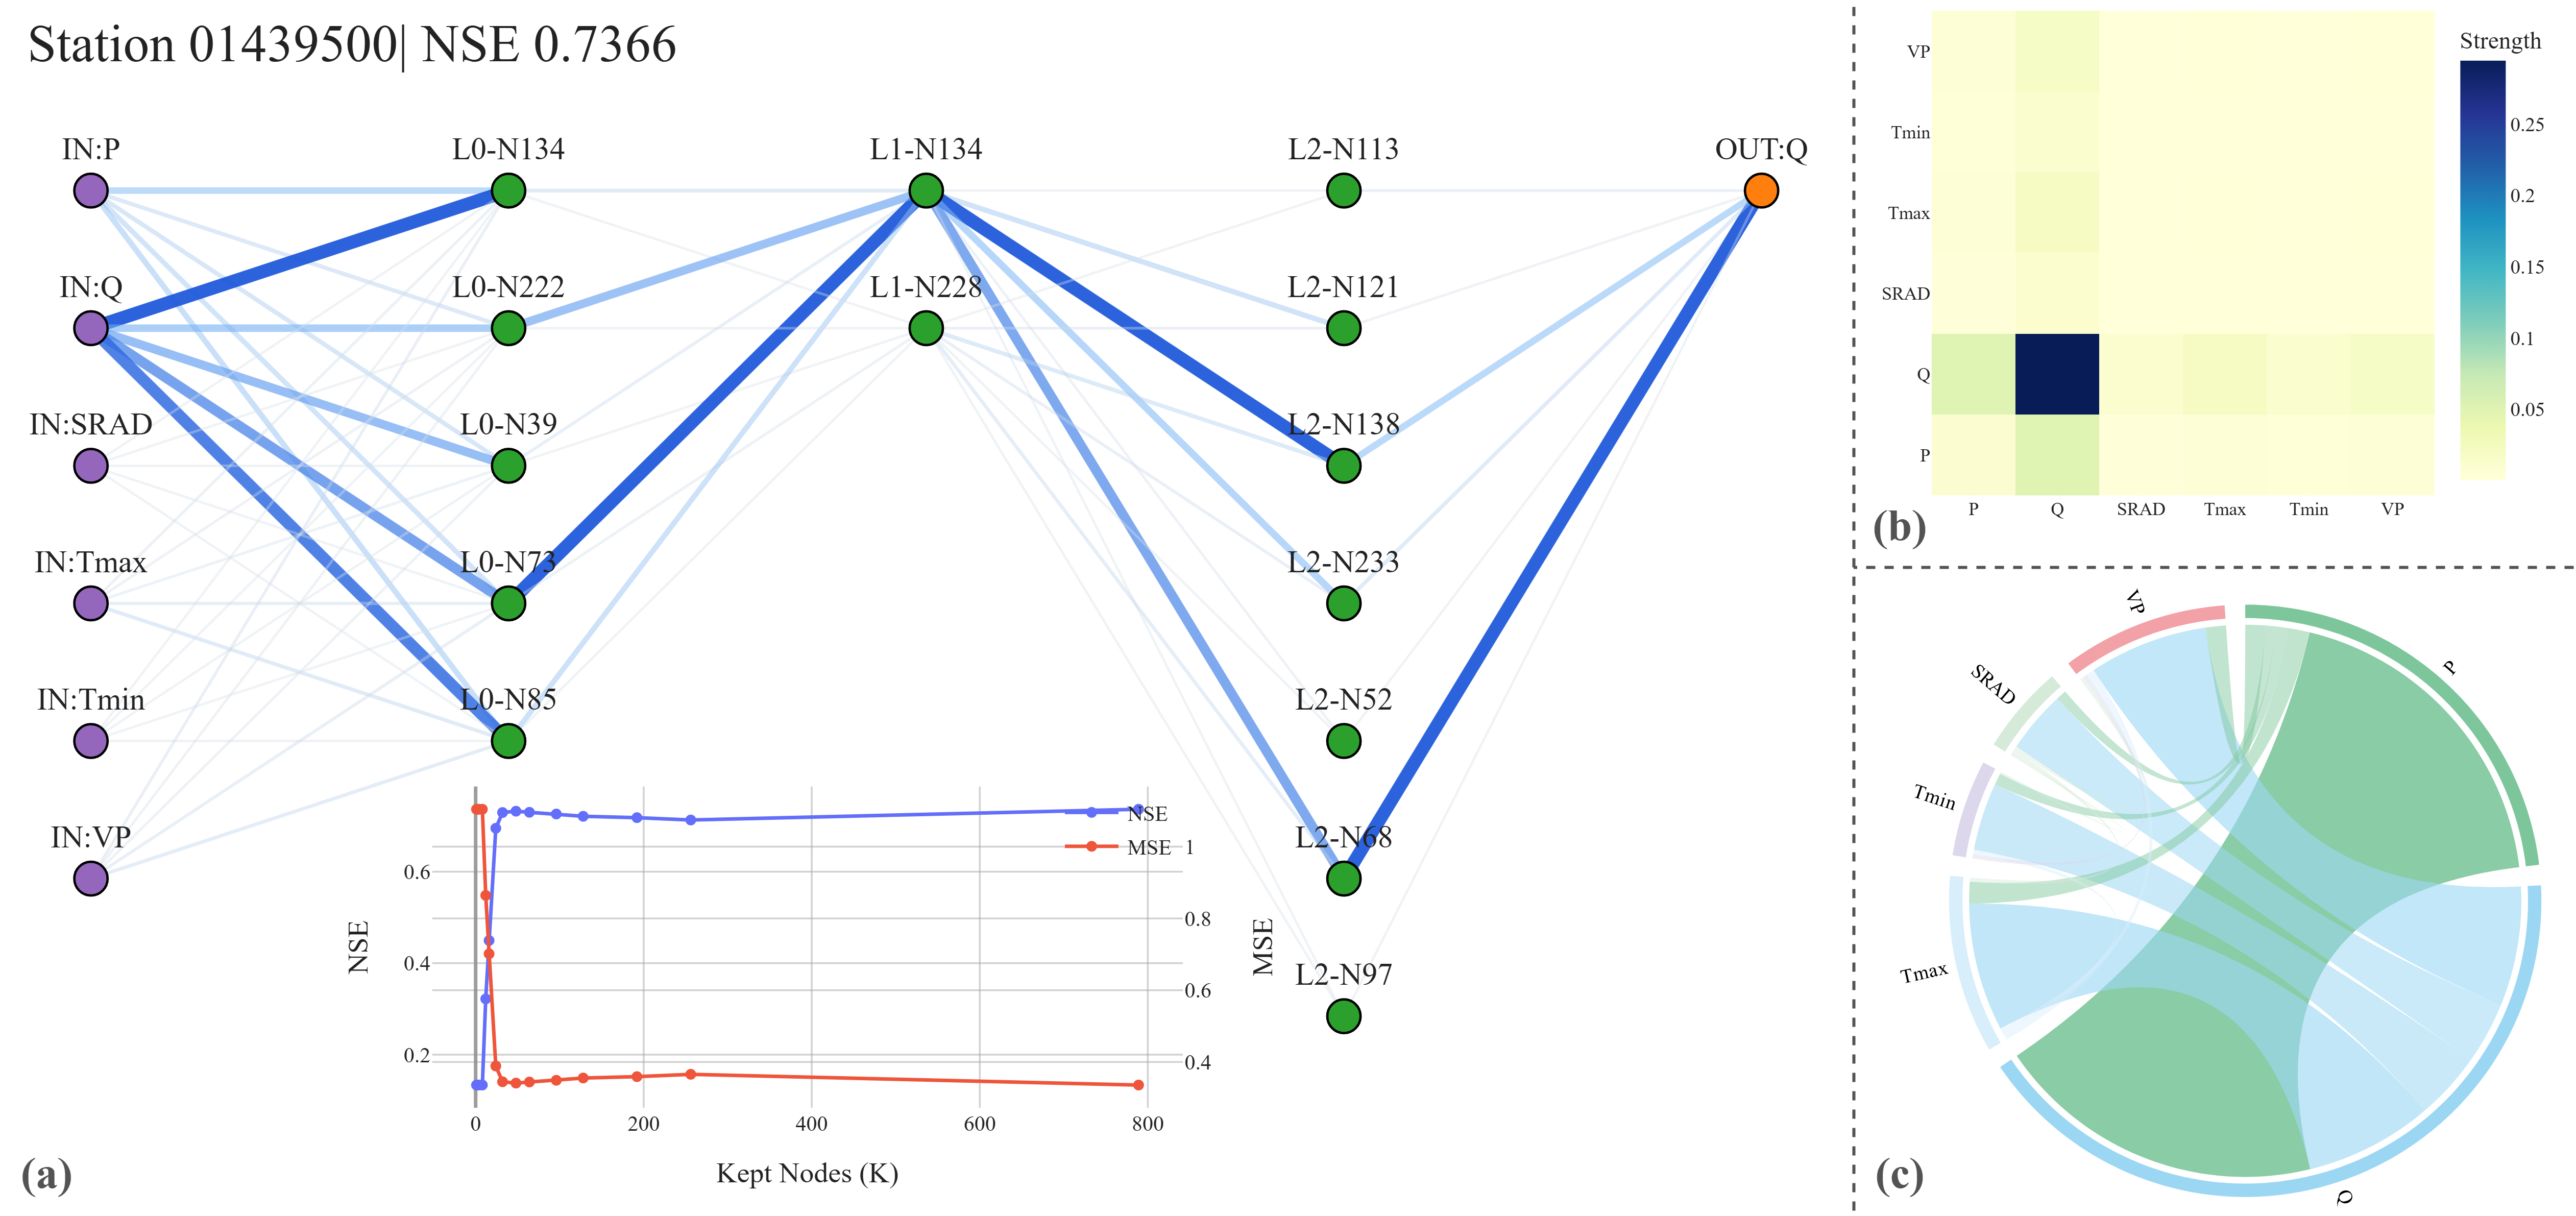
\includegraphics[width=\linewidth]{../Figures/Nse_73.png}
    \caption{Extracted sparse circuit structure and key pathways for a representative station with good performance (NSE = 0.7366).}
    \label{fig:good_station}
\end{figure}

When performance decreases further, the learned structure becomes visibly less coherent. For a representative station with satisfactory performance (Station ID: 03504000, \textit{Nantahala River near Rainbow Springs, NC}, 35.13°N, 83.62°W, NSE = 0.6217), the extracted circuit is less structured and more diffuse (Fig.~\ref{fig:satisfactory_station}). Although streamflow (Q) still dominates prediction, other variables such as radiation (SRAD) and DayL show weaker and less consistent contributions. Interaction patterns are also less pronounced, suggesting that no single robust hydrological pathway is cleanly separated from competing signals. The circuit retains more redundant connections, and sparsity-inducing training appears less effective in isolating a compact predictive core\cite{openai_weight_sparse_transformers}. This trend highlights the increasing difficulty of extracting clear and physically consistent hydrological knowledge in lower-performing cases\cite{ORTH2015147}.

\begin{figure}[ht]
    \centering
    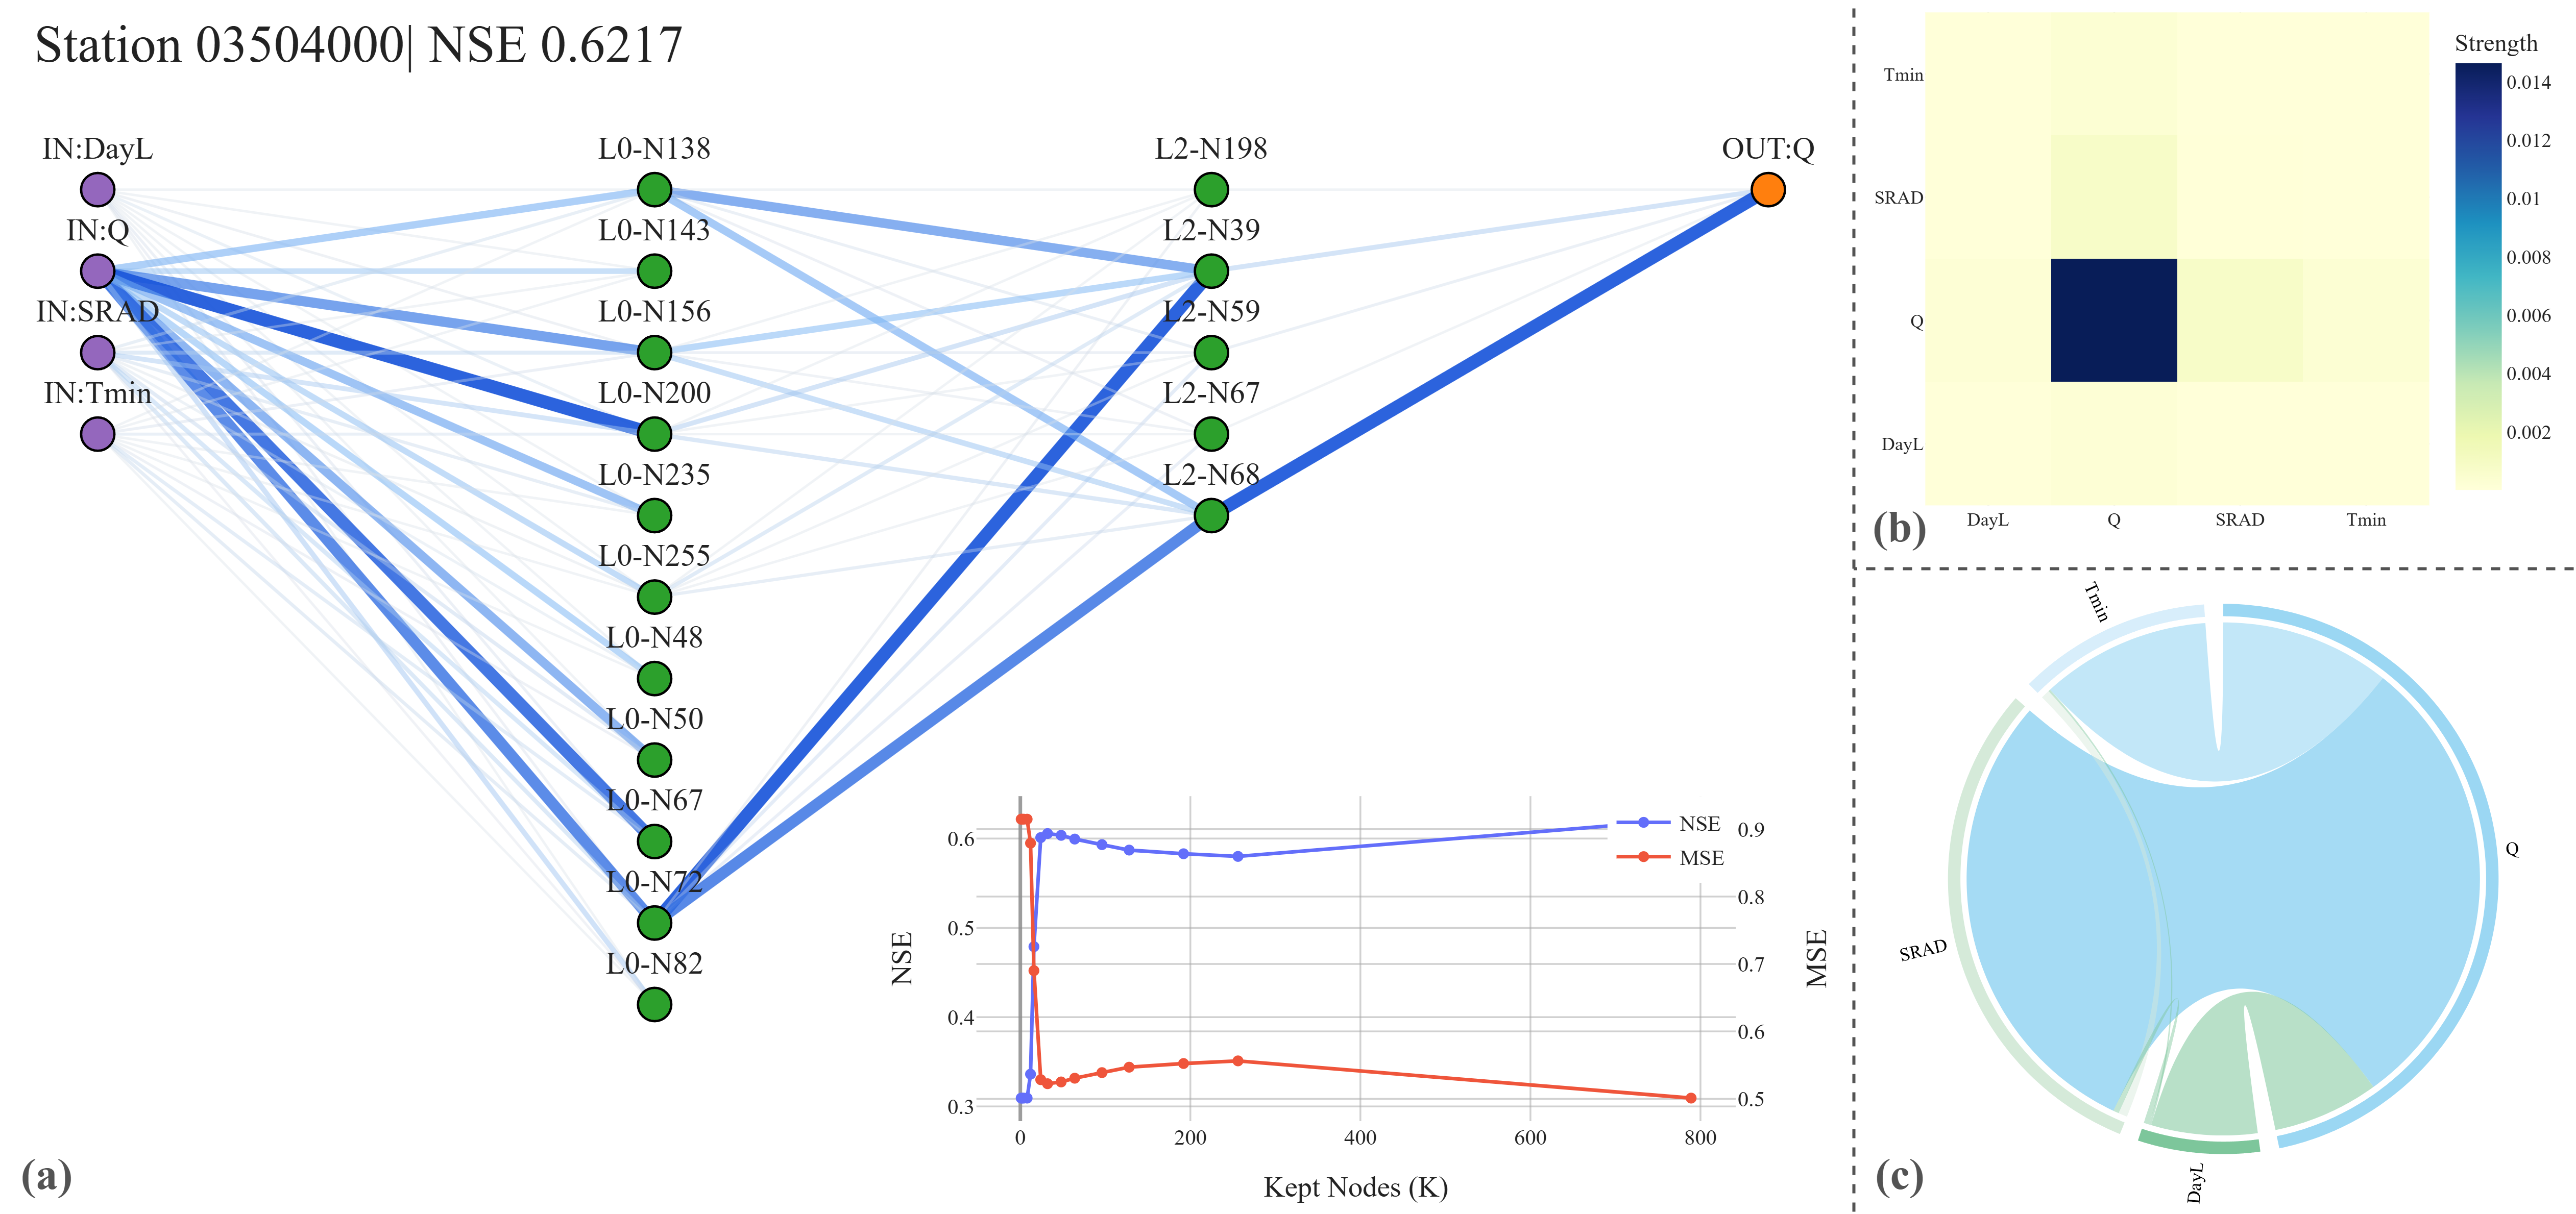
\includegraphics[width=\linewidth]{../Figures/Nse_62.png}
    \caption{Extracted sparse circuit structure and key pathways for a representative station with satisfactory performance (NSE = 0.6217).}
    \label{fig:satisfactory_station}
\end{figure}

Comparing the three representative stations, an illustrative pattern is observed: as predictive performance decreases, the extracted circuits become less sparse and more diffuse. In these cases, high-performing stations exhibit compact and structured pathways that map to identifiable hydrological modes, while lower-performing stations show increased redundancy, weaker interaction coherence, and less stable knowledge-level interpretation. 

\FloatBarrier